\chapter{Sferna trigonometrija}

Oceanska navigacija, je navigacija, ki poteka na odprtem morju in na \emph{velikih razdaljah}. Recimo tipičen primer je tako plovba med Ameriko in Azijo, kot je prikazana na sliki \ref{fig:02-01-ortodorma_loksodroma}. Na slik \ref{fig:02-01-ortodorma_loksodroma}a se takoj opazi, da je najkrajša pot tista \textit{čudna} pot, ki je na Merkatorjevi navigacijski karti (slika \ref{fig:02-01-ortodorma_loksodroma}b) prikazana kot ukrivljena pot, ki jo imenujemo \emph{Ortodroma}. 

	\begin{figure}[!htpbp]
		\begin{minipage}[t]{55mm}
			(a)
			\vspace{2mm}
			\begin{center}
				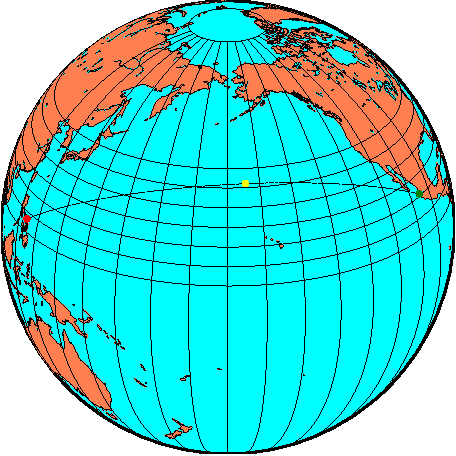
\includegraphics[width=55mm]{02_st/figs/fig_02_01-gc_path.pdf}
			\end{center}
		\end{minipage}
		\hfill
		\begin{minipage}[t]{55mm}
			(b)
			\vspace{2mm}
			\begin{center}
				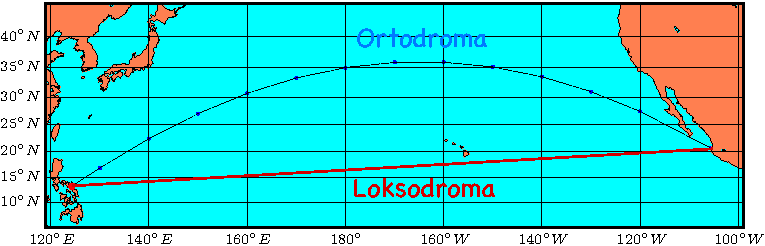
\includegraphics[width=55mm]{02_st/figs/fig_02_02-gc_RL-path.pdf}
			\end{center}
		\end{minipage}
		\caption{Prikaz razlike med potjo po krožnici--\textit{Ortodroma} in potjo po liniji--\textit{Loksodromi}, ki seka meridiane vedno pod istim kotom.}
		\label{fig:02-01-ortodorma_loksodroma}
	\end{figure}

Lepa pot med točko odhoda in točko prihoda, ki je prikazana na sliki \ref{fig:02-01-ortodorma_loksodroma}b kot ravna je ravna črta, je pot, ki ji pravimo \emph{Loksodroma}. Primera pokažeta, da je obvladovanje in razumevanje krivulj, ki potekajo po sferi, zelo pomembna vsebina na področju oceanske navigacije. 

Motivacija razlage in uporabe sferne trigonometrije je povezana predvsem z kombinacijo različnih lokov, ki potekajo po sferi. V večno primerih so loki, ki so deli \emph{velike krožnice}. Pomen le teh, bo razložen kasneje. 


\section{Kratka zgodovina razvoja}

Začetki sferne trigonometrije segajo že daleč v preteklost. Zgodovinarji pravijo, da so probleme sferne trigonometrije obravnavali že stari Indijci in Kitajci. Nam bližje je delo starih Grkov, \textit{Menelausa iz Aleksandrije}, ki v svojem delu \textit{Sphaerica} obravnava sferno trigonometrijo in prikaže razpravo o geodetkah, kjer se ukvarja z izračunom dolžine lokov, ki potekajo po sferi. Tudi zelo znan grški matematik \textit{Evklid} se je ukvarjal s problemi sferne trigonometrije. V svojih razpravah je tako pričel z osnovami razvoja kosinusnega izreka v sferni trigonometriji.

Različne razprave o sferni trigonometriji, so kasneje prispevali arabski matematiki. Recimo \textit{Abu Nasri Mansur ibn Ali ibn Iraq}, ki je bil študent zanega arabskega matematika \textit{Abū al-Wafā Būzhjānī}, je izpeljav sinusni izrek za sferni trikotnik. Kasneje so sledila še druga odkritja različnih zakonov in identitet sferne trigonometrije. Motivacija je bila določitev smeri, iz kraja opazovalca do stavbe \textit{Kabba}, ki je center muslimanske vere. To je tako imenovani problem \textit{qibla}. V tem problemu je Abu Nasri obravnaval izračun smeri, ki jo določa velika krožnica, ki povezuje kraj opazovalca in pa položaj Kabbe.

Kasneje se v obdobju razsvetljenstva v celoti postavijo aksiomatični temelji sferne trigonometrije, kakor jih poznamo danes. \emph{John Napier} je bil izjemen škotski matematik, ki je tako v 17. stoletju postavil temelje sferne trigonometrije, kot jo poznamo danes. John Napier ni znan samo po sferni trigonometriji, ampak še po obravnavi logaritmov, decimalnem zapisu števil in podobnem.

Kot vidimo skozi kratek zgodovinski opis, se je sferna trigonometrija, kot jo poznamo danes, razvijala kar nekaj časa.



\section{Osnovne definicije}

Sferna trigonometrija je eno od različnih poglavji matematike. Kot taka, mora temeljiti na osnovnih definicijah, da ja kasnejša razprava jasna in enovita. V tem poglavju bomo tako predstavili in opisali osnovne pojme, ki se pojavljajo v sferni trigonometriji.

\subsection{Velika in mala krožnica}

Pričnimo z definicijo majhne in velike krožnice, ki poteka po sferi. Kot je prikazano na sliki \ref{fig:02-02-small_great_circle} je opaziti, da je krožnica na sferi določena kot presečna krivulja med ravnino in sfero. V tem primeru ločimo dva primera:

\begin{itemize}
	\item \emphc{velika krožnica} (great circle): v tem primeru ravnina \emph{poteka skozi center sfere} in je tako presečna krivulja med ravnino in sfero vedno krožnica, ki ima radij \emph{enak} radiju sfere,
	\item \emphc{mala krožnica} (small circle): v tem primeru ravnina \emph{ne poteka skozi center sfere} in je tako presečna krivulja med ravnino in sfero vedno krožnica, ki ima radij \emph{manjši} kakor je radij sfere. 
\end{itemize}

\begin{figure}[!htpbp]
	\begin{center}
		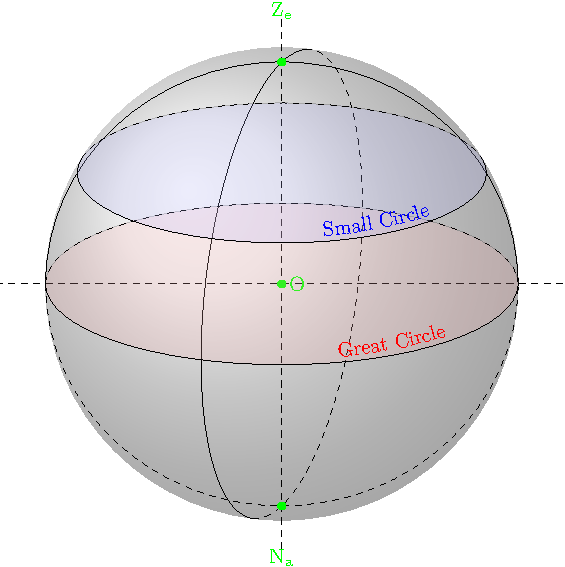
\includegraphics[width=80mm]{02_st/figs/fig_02_03-small_great_circle.pdf}
	\end{center}
	\caption{Prikaz poteka \textit{velike krožnice} (great circle -- GC) in \textit{male krožnice} (small circle -- SC) na sferi.}
	\label{fig:02-02-small_great_circle}
\end{figure}

Kot bomo videli kasneje, bo zelo pomembna definicija velike krožnice, saj je sferni trikotniki vedno sestavljen iz lokov velikih krožnic.

\subsection{Krožni lok}  

\section{Zakoni sferne trigonometrije}

Uvodne besede ...


\section{Primeri}